% Acting on the Unseen -- AAMAS/JAAMAS submission skeleton.
% NOTE: written with the standard `article` class so it compiles anywhere.
% For submission, switch to the AAMAS class, e.g. \documentclass[sigconf]{acmart}
% (or the IFAAMAS template), and move the abstract/author block accordingly.
% Figures are vector PDFs in ../figures/pdf/ (raster PNGs also in ../figures/).
\documentclass[11pt]{article}
\usepackage[margin=1in]{geometry}
\usepackage{amsmath,amssymb,amsthm}
\usepackage{graphicx}
\usepackage{booktabs}
\usepackage[hidelinks]{hyperref}
\usepackage{xcolor}

\theoremstyle{plain}
\newtheorem{theorem}{Theorem}
\newtheorem{lemma}{Lemma}
\newtheorem{corollary}{Corollary}

\title{Acting on the Unseen: Collaborative Filtering for Decentralized
Multi-Robot Task Allocation under Minimal Assumptions}
\author{Yigal Meshulam \and Alexander Apartsin}
\date{}

\begin{document}
\maketitle

\begin{abstract}
We study multi-robot task allocation under the least possible information: a swarm
with no prior knowledge (not even the problem's rank), zero communication, only
partial and noisy observation of a public outcome stream, and fully distributed
decisions. We show that, even so, each agent can act well on tasks it has never
tried, onboard brand-new tasks, and welcome new agents, by running online
collaborative filtering over the public broadcast. Against any structure-free
learner this is a \emph{categorical} separation (the structure-free learner is at
the error floor on unseen pairs by construction); we prove a matching per-agent
sample-complexity result ($\Theta(d)$ vs.\ $\Theta(n)$) and an anytime
(cumulative-reward) separation. Against a broad, fairly-constrained field of
low-rank and structured methods, our online, masking-robust, anytime-optimal
estimators dominate throughout the limited-observability regime, and the advantage
transfers to an independent simulator.
\end{abstract}

\section{Introduction}
\textbf{Minimal assumptions.} No prior knowledge. Zero communication. Only partial,
noisy observables. Fully distributed decisions. Can a swarm still act intelligently,
in particular on the unseen? We answer yes, and prove the advantage is categorical.

A swarm repeatedly chooses which target to engage; agent-target compatibility is
hidden but low-rank, there are far more targets than rounds ($n \gg T$), agents do
not coordinate or share parameters, and each senses only a noisy, partial slice of
the public outcomes. The crux is generalization: a structure-free learner that
estimates a target only from its own engagements is, on any target it never touched,
at the prior-mean error floor, which dominates under starvation.

\textbf{Contributions.} (1) A minimal-assumption, decentralized, online,
broadcast-only formulation of collaborative filtering (CF) for MRTA. (2) The
categorical unseen-pair and onboarding/cold-start results ($\Theta(d)$ vs
$\Theta(n)$). (3) An anytime separation under sample starvation. (4) A masking-model
dichotomy (durable vs transient decentralization) and an additive rank-ceiling
result. (5) A method family that is masking-robust and anytime-optimal, dominating
prior-art low-rank methods, plus collective active exploration; validated in a
independent simulator. An interactive tutorial with all figures and proofs is
public.\footnote{\url{https://apartsinprojects.github.io/ZKDroneSwarm/tutorial.html}}

\section{Problem statement}
\textbf{World.} $m$ drones, $n$ targets, with $K_1/K_2$ latent types. Reward is the
cosine of unit latent factors, $R_{ij} = \langle p_i, u_j\rangle \in [-1,1]$,
genuinely rank $d = \min(d,K_1,K_2)$ (a bilinear form; no nonlinear link).

\textbf{Observation (communication-free).} A public stream carries each engagement's
(action, outcome). Drone $i$ senses its own outcome cleanly (noise $\sigma_{\text{own}}$)
and a per-drone-limited, noisy slice of teammates' outcomes: a mask keeps teammate
$k$ with probability $\rho$ (persistent or i.i.d.), with reward noise $\sigma_{\text{obs}}$.
This is passive sensing of public outcomes, not transmission; there is no message
passing, no parameter sharing, and no coordinator.

\textbf{Baselines.} Structure-free: Random, UCB-Indep (per-(drone,target) UCB1),
UCB-Homogeneous (shared arm table), Tabular. Low-rank/structured: SGD-MF, ESTR
(explore-then-spectral) \cite{jun2019bilinear}, probe-then-fit, BPMF
\cite{salakhutdinov2008bayesian}, SoftImpute \cite{mazumder2010spectral}, memory-based
$k$NN-CF, and an additive bias model \cite{koren2009matrix}. Every method is an
independent per-drone learner with a guessed rank $\hat d$ (or none), the same noisy
partial stream, and no parameter sharing; the \emph{oracle} (centralized, complete
information) is used only to normalize scores.

\textbf{Metrics.} For drone $i$ offered a uniform size-$c$ set each round, let
$\mu_i$ be its mean reward and $\rho^{\text{or}}_i = \mathbb{E}_S[\max_{j\in S} R_{ij}]$.
A policy with expected earned reward $\rho$ has
$\mathrm{skill} = (\rho-\mu_i)/(\rho^{\text{or}}_i-\mu_i)$ (0 = random, 1 = oracle).
\emph{Unseen-pair skill} restricts to targets $i$ never pulled. \emph{Anytime skill}
is the cumulative normalized reward over rounds (charges any probe phase).
\emph{State-uniqueness} is the divergence of agents' learned reward matrices.

\section{Method}
Each agent runs its own online weighted alternating least squares over the events it
senses, weighting each by precision $1/\sigma^2$ (a masked event has zero precision,
not zero value, the key to masking-robustness) \cite{hu2008collaborative}; estimation
is separated from the decision policy. We foreground \textbf{ActiveCF}: a
latent-space UCB (predicted reward plus a broadcast count-based uncertainty bonus, so
one agent's probe lowers everyone's uncertainty -- collective active learning). We
ablate RewardCF (rewards only; anytime-optimal), ChoiceZK (actions only; noise-immune
fallback), and HybridCF (probe, SVD warm-start, then online weighted-ALS; best
final-policy unseen).

\section{Theory}
Proof sketches in the supplement; each result is mapped to a confirming experiment.
\begin{theorem}[Tabular floor]\label{t1}
A structure-free learner has expected squared error $\Omega(\mathrm{Var}_j R_{ij})$
on any never-observed pair and unseen-pair skill $0$; the broadcast is uninformative
to it. Pooling recovers only the rank-1 popularity term.
\end{theorem}
\begin{theorem}[CF row completion]\label{t2}
If the target factors $U$ (rank $d$) are known and drone $i$ observes $\ge d$ rewards
whose factors span $\mathbb{R}^d$, its entire row is recovered exactly by a least-squares
fold-in (with i.i.d.\ noise of variance $\sigma^2$, the per-target prediction error is
$O(\sigma^2 d / \lambda_{\min}(U_\Omega^\top U_\Omega))$). $U$ itself is identified from
the pooled broadcast by standard \emph{incoherent} low-rank matrix completion from
$\tilde O(d(m+n))$ entries \cite{candes2009exact,keshavan2010matrix,recht2011simpler};
the fold-in is the per-agent step. Per-agent $\Theta(d)$ vs tabular $\Theta(n)$:
categorical on unseen pairs.
\end{theorem}
\begin{theorem}[Anytime separation]\label{t3}
For $n\gg T$, any structure-free learner's anytime skill is $\le g(cT/n)\to 0$ (even
with full broadcast), where $g$ is the expected-order-statistic gap; a CF learner
reaches near-oracle in $O(d)$ rounds. The closed-form ceiling is informative in the
\emph{starved} regime $cT \ll n$; at any operating point the sharper, exact mechanism
is that a never-tried target carries an unbounded exploration bonus, so a per-arm
learner pulls an untried target whenever its offer contains one (probability $\to 1$
while the number of distinct pulls $\ll n$) and earns $\approx$ random throughout.
\end{theorem}
\begin{theorem}[Masking dichotomy]\label{t4}
Under i.i.d.\ loss every agent eventually senses everything (Borel--Cantelli) so
models converge (transient heterogeneity); under persistent masking each agent has a
permanent blind set so models stay distinct (durable). The unseen and anytime
results are invariant to the choice.
\end{theorem}
\begin{theorem}[Additive ceiling]\label{t5}
An additive predictor $a+b_i+c_j$ has rank $\le 2$ and reduces to the popularity
order, so its unseen skill is strictly below CF for $d>1$.
\end{theorem}
Standard matrix-completion bounds \cite{candes2009exact,keshavan2010matrix,recht2011simpler}
are centralized and about estimation error; ours are per-agent, online, broadcast-only,
with the unseen-pair floor making the gap categorical, plus the anytime separation.

\section{Experiments}
\textbf{Categorical (Fig.~\ref{fig:unseen}).} CF acts well on never-observed pairs at
every density while structure-free learners sit at the floor; new targets and new
agents are absorbed from $\sim d$ probes vs $\sim n$.
\textbf{Anytime (Fig.~\ref{fig:anytime}).} On earned reward our online methods
dominate at every horizon; per-arm bandits stay near random under $n\gg T$.
\textbf{Versus the field.} With a converged estimator our methods dominate the
strongest competitors (PTF, SoftImpute) under masking and on anytime
(Fig.~\ref{fig:pareto}); SoftImpute leads only dense-broadcast unseen.
\textbf{Robustness.} Results are invariant to the masking model and degrade
gracefully as the world leaves exact low-rank; the advantage transfers to the
independent tabula\_drone simulator (skill $\approx 0.81$, beating the env's SGD-MF and
UCB-Indep, approaching the oracle).

\textbf{Scope (when CF beats structure-free).} The advantage is not universal; across a
structure$\times$observability grid it holds \emph{iff} three conditions co-occur.
(i) The reward is low-rank but \emph{personalized}, $1<d\ll\min(m,n)$: at $d=1$ the
reward is a shared popularity order a pooling/bias baseline already captures (Thm.~\ref{t5}),
and at $d\to\min(m,n)$ there is no structure to exploit (graceful collapse, F14).
(ii) The regime is \emph{sample-starved}, $n\gg cT$: when sample-rich, a tabular learner
eventually measures every entry and the unseen advantage vanishes (scaling sweeps).
(iii) The reward channel is \emph{shared}, $\rho>0$: without a broadcast each agent has
only its own data and CF degenerates to tabular. This scopes the claim and explains why
structure-free methods are competitive in sample-rich, low-personalization, or unshared
settings (our earlier null results).

\begin{figure}[t]\centering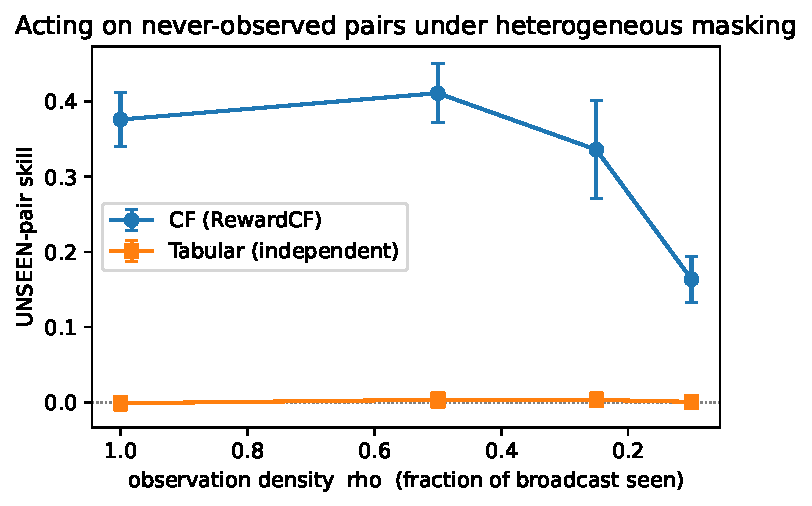
\includegraphics[width=0.7\linewidth]{../figures/pdf/F2_unseen_masking.pdf}
\caption{Unseen-pair skill vs observation density (categorical separation).}\label{fig:unseen}\end{figure}
\begin{figure}[t]\centering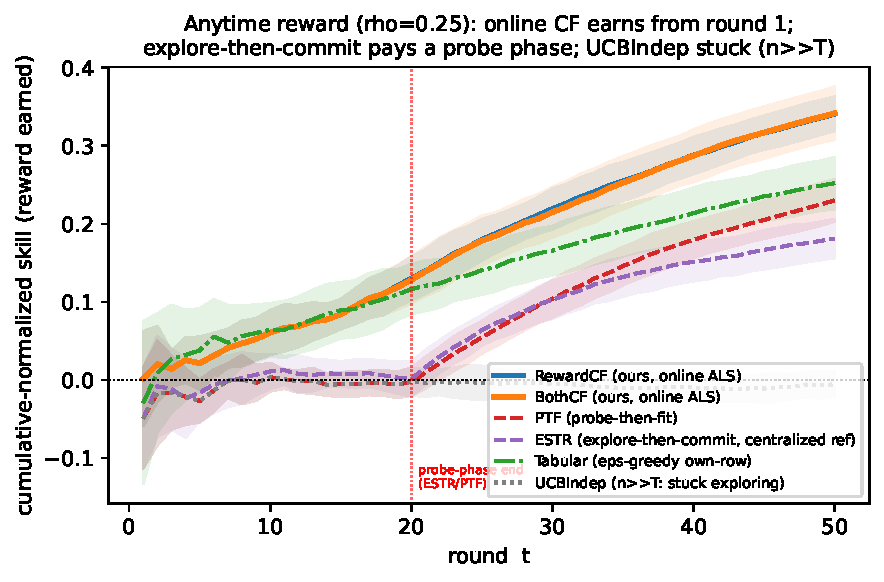
\includegraphics[width=0.7\linewidth]{../figures/pdf/F6_anytime.pdf}
\caption{Anytime cumulative reward: online CF earns from round one.}\label{fig:anytime}\end{figure}
\begin{figure}[t]\centering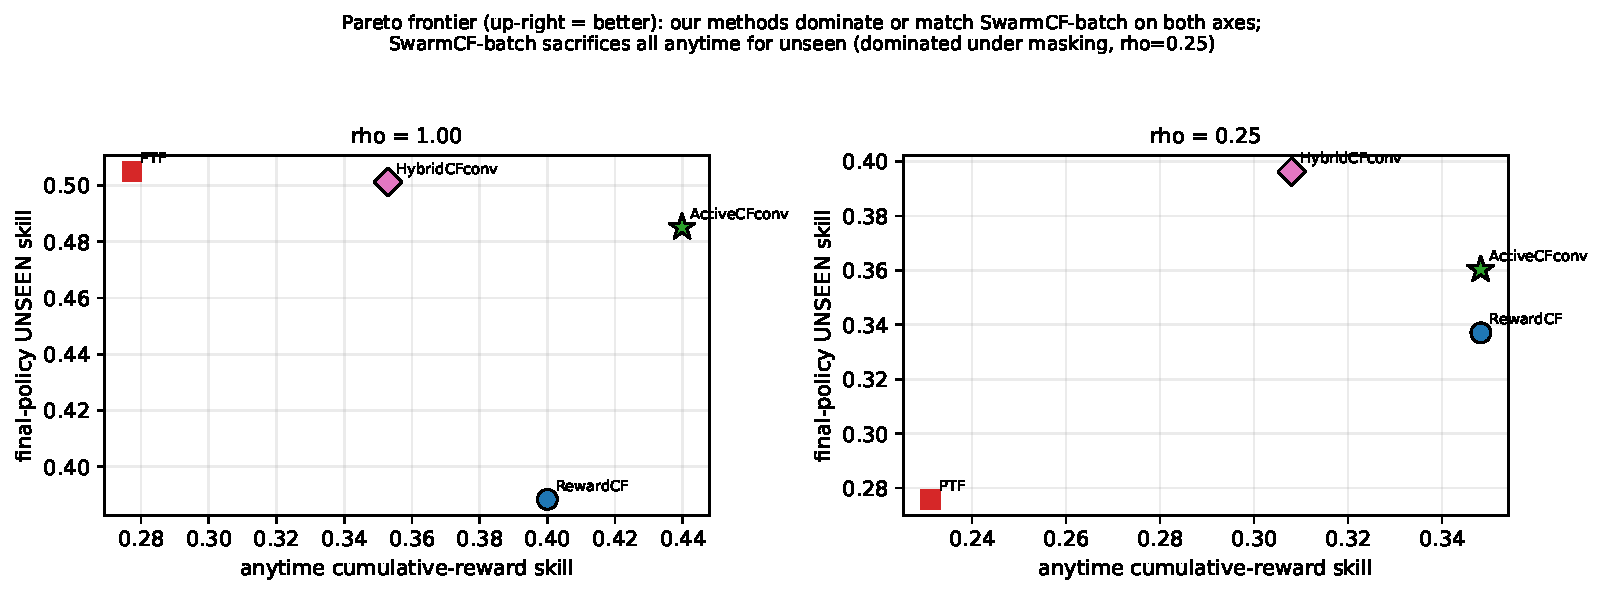
\includegraphics[width=0.8\linewidth]{../figures/pdf/F11_pareto.pdf}
\caption{Pareto frontier (anytime vs unseen): our methods dominate.}\label{fig:pareto}\end{figure}

\section{Related work}
Matrix completion \cite{candes2009exact,keshavan2010matrix,recht2011simpler,mazumder2010spectral}
gives the centralized statistical backbone; we make it decentralized, online, and
broadcast-only. Low-rank and contextual bandits
\cite{jun2019bilinear,li2010contextual,chapelle2011empirical} and online clustering of
bandits \cite{gentile2014online} are centralized and/or phase-structured; we are
anytime and distributed. Recommender CF \cite{koren2009matrix,hu2008collaborative,
salakhutdinov2008bayesian} inspires our estimator and the exposure-debiased choice
channel. We connect to the MRTA taxonomy \cite{gerkey2004formal} and decentralized
MARL, but remove communication, priors, and shared state.

\section{Limitations and conclusion}
\textbf{Scope: contention.} Our formal results assume non-contention. We tested hard
contention directly (capacity-1 matching: a shared pool, each target awarded to one
random contender, earned reward normalized by the Hungarian optimum, pool swept
$240\to15$). Three findings. (i) The \emph{categorical} unseen-pair result SURVIVES:
preference quality (evaluated contention-free after training) stays high for CF
($\approx0.29$-$0.38$) versus the structure-free floor ($\approx0$) at every pool size,
since it is a property of the learned model. (ii) On \emph{operational} earned reward CF
already beats the field at low/moderate contention; greedy (argmax) CF collapses toward
the matching floor only at severe contention. (iii) We WIN even there with a one-line
decentralized fix, ContentionCF (the CF estimate plus a FIXED private per-target offset
for deterministic symmetry breaking): at pool $=15$ it earns $0.105\,[0.096,0.114]$ versus
$\approx0.05$ for argmax-CF/PTF (non-overlapping, $\sim2\times$), with no communication;
it is regime-dependent (helps once collisions bind), so a collision-rate-adaptive offset
would dominate. (iv) De-confliction must use \emph{private, fixed} randomness: per-round
softmax and shared-signal (popularity / collective count-bonus) routing both backfire by
re-colliding or re-synchronizing.
Consistent soft-contention evidence: the independent tabula\_drone validation runs with
HP depletion and our method still leads (skill $\approx 0.81$).

Under minimal assumptions, CF over the public broadcast lets a swarm act on the unseen,
onboard new tasks and agents, and earn from the first round, with a categorical,
theory-backed advantage and dominance over prior-art low-rank methods in the
limited-observability regime.

\paragraph{Reproducibility.} All numbers derive from complete per-seed data; figures
and this paper are regenerable. Code, data, proofs, and the tutorial:
\url{https://github.com/ApartsinProjects/ZKDroneSwarm}.

\bibliographystyle{plain}
\bibliography{references}
\end{document}
